\documentclass[aspectratio=43]{beamer}

% ===== TEMA BASADO EN PLANTILLA.PPTX CON IMÁGENES =====
\usepackage[utf8]{inputenc}
\usepackage[spanish]{babel}
\usepackage{graphicx}
\usepackage{physics}
\usepackage{tikz}
\usepackage{amsmath}
\usepackage{amssymb}
\usepackage{algorithm}
\usepackage{algpseudocode}
\usepackage{booktabs}
\usepackage{hyperref}

% Configuración de tema limpio sin decoraciones por defecto
\usetheme{default}
\usecolortheme{default}

% Colores extraídos de la plantilla PPTX
\definecolor{azuloscuro}{RGB}{54,80,255}       % rgba(54, 80, 255, 1)
\definecolor{azulclaro}{RGB}{112,114,225}    % rgba(112, 114, 255, 1)
\definecolor{grisclaro}{RGB}{237,237,237}   % rgba(237, 237, 237, 1)
\definecolor{naranjaacento}{RGB}{134,78,255}  % rgba(134, 78, 255, 1)

% Configuración de colores
\setbeamercolor{structure}{fg=azuloscuro}
\setbeamercolor{frametitle}{fg=azuloscuro}
\setbeamercolor{block title}{bg=azulclaro,fg=white}
\setbeamercolor{block body}{bg=grisclaro,fg=black}
\setbeamercolor{block title alerted}{bg=naranjaacento,fg=white}
\setbeamercolor{block body alerted}{bg=naranjaacento!15,fg=black}

% ===== CONFIGURACIÓN DE BLOQUES =====
\setbeamertemplate{blocks}[rounded][shadow=false]
\setbeamerfont{block title}{size=\normalsize,series=\bfseries}
\setbeamerfont{block body}{size=\normalsize}
\setbeamercovered{transparent}

% ===== CONFIGURACIÓN DE ITEMIZE/ENUMERATE =====
\setbeamertemplate{itemize items}[circle]
\setbeamertemplate{enumerate items}[default]
\setbeamercolor{item}{fg=azulclaro}
\setbeamercolor{subitem}{fg=azulclaro!10}
\setbeamercolor{itemize/enumerate body}{fg=black}

% ===== FONDO DE DIAPOSITIVA =====
% Fondo diferente para título (image3) y contenido (image8)
\setbeamertemplate{background}{%
  \begin{tikzpicture}[remember picture,overlay]
    % Fondo principal: image3 para título, image8 para contenido
    \ifnum\value{framenumber}=1
      \node[at=(current page.center),opacity=1.0] {
        \includegraphics[width=\paperwidth,height=\paperheight]{pptx_media/image3.png}
      };
    \else
      \node[at=(current page.center),opacity=1.0] {
        \includegraphics[width=\paperwidth,height=\paperheight]{pptx_media/image8.png}
      };
      % Sello en esquina superior derecha (image9) - solo en diapositivas de contenido
      \node[anchor=north east,inner sep=0.25cm] at (current page.north east) {
        \includegraphics[width=1.5cm]{pptx_media/image9.png}
      };
    \fi
  \end{tikzpicture}%
}

% ===== PIE DE PÁGINA CON IMAGEN =====
\setbeamertemplate{footline}{
  \begin{tikzpicture}[remember picture,overlay]
    % Fondo del footer (foot_bkg.png)
    \node[anchor=south west,inner sep=0pt] at (current page.south west) {
      \includegraphics[width=\paperwidth,height=0.7cm]{pptx_media/foot_bkg.png}
    };
    % Imagen del footer encima del fondo (image5.png)
    \node[anchor=south west,inner sep=0pt] at (current page.south west) {
      \includegraphics[width=\paperwidth,height=0.7cm]{pptx_media/image5.png}
    };
    % Texto sobre el footer (solo después de la primera diapositiva)
    \ifnum\value{framenumber}>1
      \node[anchor=south west,text=black] at ([xshift=0.5cm,yshift=9.2cm]current page.south west) {
        \tiny\insertshortauthor
      };
      \node[anchor=south,text=black] at ([yshift=9.2cm]current page.south) {
        \tiny\insertshorttitle
      };
      \node[anchor=south east,text=black] at ([xshift=-0.5cm,yshift=9.2cm]current page.south east) {
        \tiny\insertframenumber{}/\inserttotalframenumber
      };
    \fi
  \end{tikzpicture}%
}

% ===== ENCABEZADO VACÍO (sin navegación) =====
\setbeamertemplate{headline}{}

% Remover símbolos de navegación
\setbeamertemplate{navigation symbols}{}

% ===== CONFIGURACIÓN DE FRAMETITLE =====
\setbeamertemplate{frametitle}{
  \vspace{0.5cm}
  \begin{beamercolorbox}[wd=\paperwidth,leftskip=1cm]{frametitle}
    \usebeamerfont{frametitle}\Large\bfseries\insertframetitle
  \end{beamercolorbox}
}

% ===== TRANSPARENCIAS =====
\setbeamercovered{transparent=15}

% ===== CONFIGURACIÓN DE COLORES PARA TÍTULO Y CONTENIDO =====
% Colores para la diapositiva de título (fondo oscuro)
\setbeamercolor{title}{fg=white}
\setbeamercolor{subtitle}{fg=white}
\setbeamercolor{author}{fg=white}
\setbeamercolor{institute}{fg=white}
\setbeamercolor{date}{fg=white}

% ===== INFORMACIÓN DEL DOCUMENTO =====
\title[QML para b-Tagging]{QML con Angle Embedding y DNN\\para b-Tagging en Jets de Bajo Momento}
\subtitle{Comparación de técnicas cuánticas y clásicas en el régimen de bajo \texorpdfstring{$p_T$}{pT}}
\author[J. Montoya]{Juan Montoya}
\institute[UdeA]{
  Instituto de Física\\
  Universidad de Antioquia\\
}
\date[2 Oct 2025]{2 de octubre de 2025}

% ===== COMANDOS PERSONALIZADOS =====
\newcommand{\pt}{\ensuremath{p_T}}
\newcommand{\GeV}{\text{ GeV}}
\newcommand{\pT}{\ensuremath{p_{\text{T}}}}

% ===== INICIO DEL DOCUMENTO =====
\begin{document}

% ===== DIAPOSITIVA DE TÍTULO =====
\begin{frame}
  \titlepage
\end{frame}

% ===== TABLA DE CONTENIDOS =====
\begin{frame}{Estructura de la Presentación}
  \tableofcontents
\end{frame}

% ===================================================================
% SECCIÓN 1: INTRODUCCIÓN
% ===================================================================
\section{Introducción}

% ----- Diapositiva: ¿Qué son los Jets? -----
\begin{frame}{¿Qué son los Jets?}
  \begin{columns}
    \begin{column}{0.47\textwidth}
      \begin{block}{Definición}
        \begin{itemize}
          \item Chorros colimados de partículas
          \item Producidos en hadronización
        \end{itemize}
      \end{block}
      
      \begin{alertblock}{Desafío del b-tagging}
        \begin{itemize}
          \item Identificar jets de quarks b
          \item Problemas con jets de \texorpdfstring{$p_T$}{pT} menor a 20 GeV
        \end{itemize}
      \end{alertblock}
    \end{column}
    
    \begin{column}{0.55\textwidth}
      \begin{figure}
        \centering
        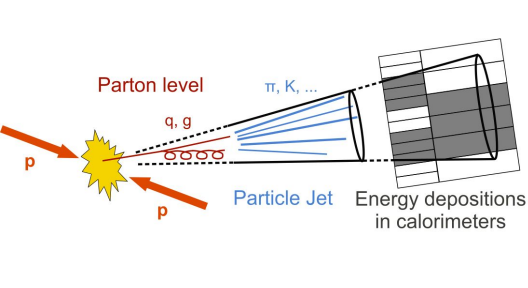
\includegraphics[width=\textwidth]{jet1.png}
        \caption{Estructura típica de un jet}
      \end{figure}
    \end{column}
  \end{columns}
\end{frame}

% ----- Diapositiva: El Reto del Bajo Momento -----
\begin{frame}{El reto del bajo momento}
  \begin{columns}
    \begin{column}{0.49\textwidth}
      \begin{block}{Régimen de \texorpdfstring{$p_T$}{pT} $<20$ GeV}
        \begin{itemize}
          \item Alta densidad de partículas
          \item Baja resolución de trazas
        \end{itemize}
      \end{block}
      \vspace{-0.3em}
      \begin{figure}
        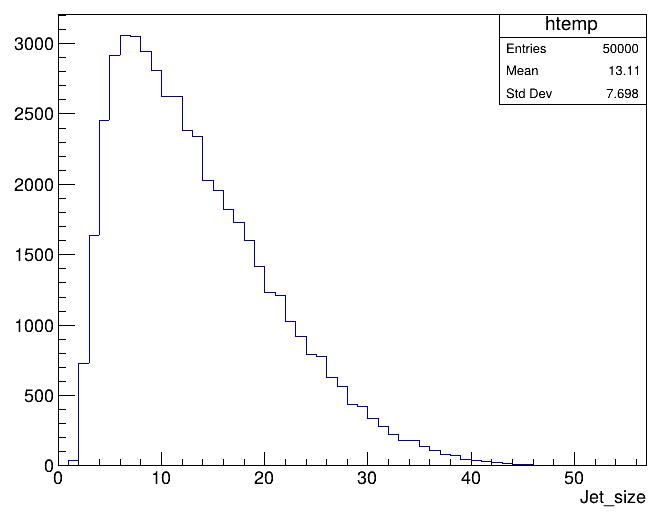
\includegraphics[width=0.79\textwidth]{njetl.png}
        \caption{\small Distribución de jets de bajo \texorpdfstring{$p_T$}{pT}}
      \end{figure}
    \end{column}
    \begin{column}{0.49\textwidth}
      \begin{block}{Importancia}
        \begin{itemize}
          \item Acceso a nueva física
          \item Nuevas metodologías
        \end{itemize}
      \end{block}
      \vspace{-0.005em}
      \begin{figure}
        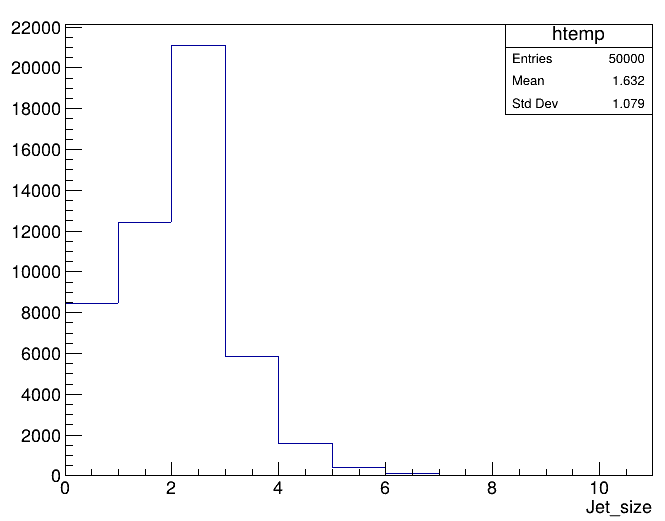
\includegraphics[width=0.79\textwidth]{njeth.png}
        \caption{\small Comparación con alto \texorpdfstring{$p_T$}{pT}}
      \end{figure}
    \end{column}
  \end{columns}
\end{frame}

% ----- Diapositiva: Comparativa Visual -----
\begin{frame}{Comparativa visual: alto vs bajo \texorpdfstring{$p_T$}{pT}}
  \vspace{-1.5em}
  \begin{block}{Diferencias}
    \begin{itemize}
      \item Estrucutra interna
      \item Calidad de reconstrucción
    \end{itemize}
  \end{block}
  
  \vspace{-0.5em}
  \begin{figure}
    \centering
    \begin{minipage}{0.49\textwidth}
      \centering
      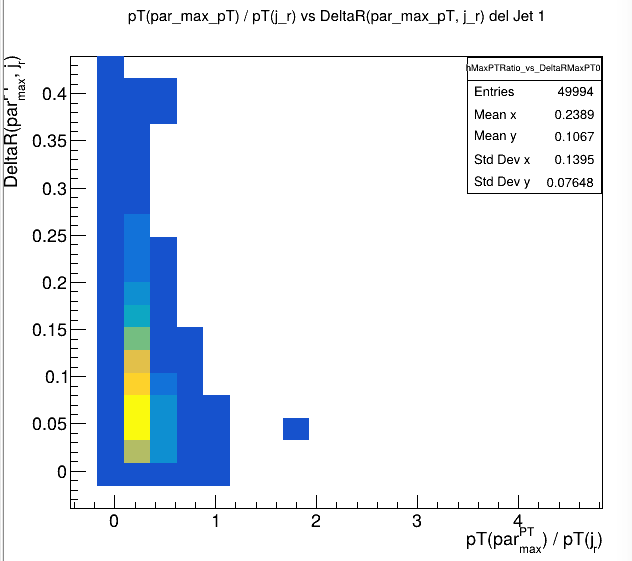
\includegraphics[width=0.75\textwidth]{lowptjet.png}
    \end{minipage}
    \hfill
    \begin{minipage}{0.49\textwidth}
      \centering
      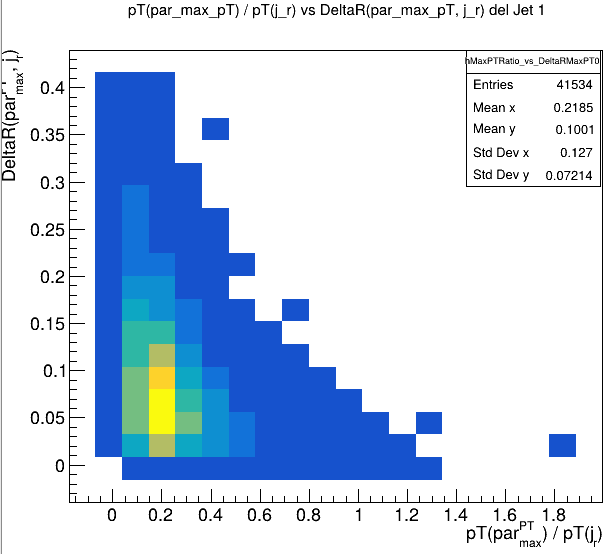
\includegraphics[width=0.75\textwidth]{higptjet.png}
    \end{minipage}
    \caption{\footnotesize Izquierda: Jet de bajo \texorpdfstring{$p_T$}{pT} ($<20$ GeV). 
    Derecha: Jet de alto \texorpdfstring{$p_T$}{pT} ($>20$ GeV)}
  \end{figure}
\end{frame}

% ----- Diapositiva: Motivación para QML -----
\begin{frame}{Motivación para QML}
  \begin{columns}[T]
    \begin{column}{0.5\textwidth}
      \begin{alertblock}{¿Por qué QML?}
        \begin{itemize}
          \item Potencial para correlaciones complejas
          \item Exploración eficiente de espacios de alta dimensión
        \end{itemize}
      \end{alertblock}
    \end{column}
    
    \begin{column}{0.5\textwidth}
      \begin{figure}
        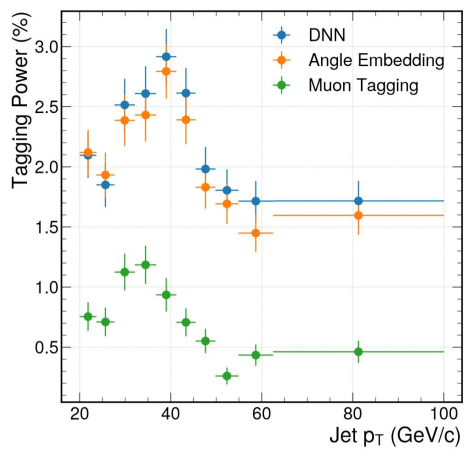
\includegraphics[width=\textwidth]{motiv.png}
        \caption{Ventaja potencial de QML}
      \end{figure}
    \end{column}
  \end{columns}
\end{frame}

% ===================================================================
% SECCIÓN 2: QUANTUM MACHINE LEARNING
% ===================================================================
\section{Quantum Machine Learning}

% ----- Diapositiva: Fundamentos de QML -----
\begin{frame}{Fundamentos de QML}
  \begin{columns}
    \begin{column}{0.5\textwidth}
      \begin{block}{Características clave}
        \begin{itemize}
          \item Computación híbrida cuántico-clásica
          \item Circuitos variacionales parametrizados
          \item Optimización clásica de parámetros
        \end{itemize}
      \end{block}
      \begin{alertblock}{Ventajas potenciales}
        \begin{itemize}
          \item Superposición cuántica
          \item Entrelazamiento de estados
        \end{itemize}
      \end{alertblock}
    \end{column}
    \begin{column}{0.5\textwidth}
      \begin{figure}
        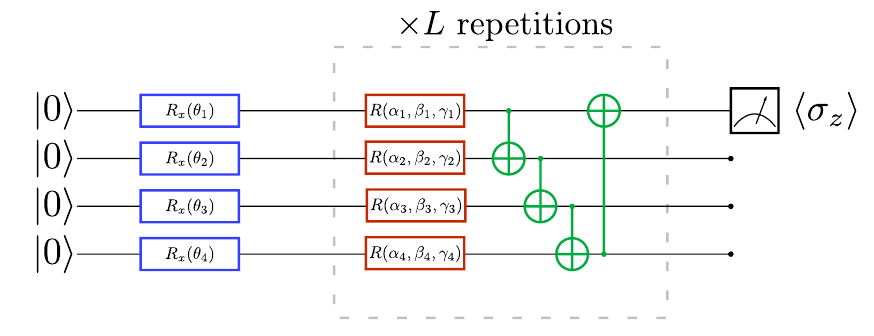
\includegraphics[width=\textwidth]{angleemb.png}
        \caption{Esquema QML}
      \end{figure}
    \end{column}
  \end{columns}
\end{frame}

% ----- Diapositiva: Angle Embedding Concepto -----
\begin{frame}{Angle Embedding: Concepto}
  \begin{columns}
    \begin{column}{0.4\textwidth}
      \begin{block}{Fundamentos}
        Para un vector de características $\mathbf{x}=[x_1,\dots,x_n]$:
        \begin{itemize}
          \item Normalización en $[-\pi,\pi]$
          \item Un qubit por característica
          \item Rotaciones $RX(x_i)$ o $RY(x_i)$
        \end{itemize}
      \end{block}
    \end{column}
    \begin{column}{0.6\textwidth}
      \begin{figure}
        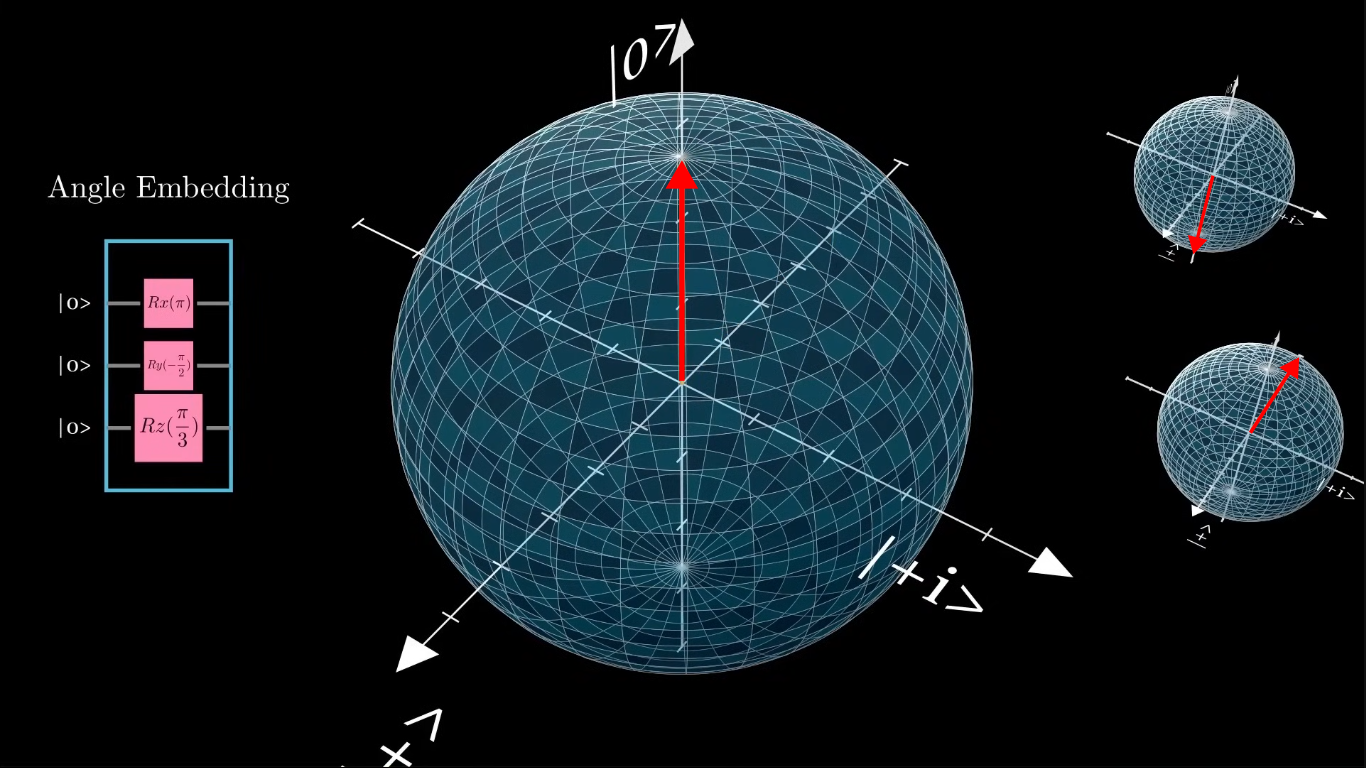
\includegraphics[width=\textwidth]{blochh.png}
        \caption{Representación en esfera de Bloch}
      \end{figure}
    \end{column}
  \end{columns}
\end{frame}

% ----- Diapositiva: Aplicación al b-tagging -----
\begin{frame}{Aplicación al b-tagging}
  \begin{columns}
    \begin{column}{0.45\textwidth}
      \begin{block}{16 Características del Jet}
        \begin{itemize}
          \item Variables cinemáticas (\texorpdfstring{$p_T$}{pT}, \texorpdfstring{$\eta$}{eta}, \texorpdfstring{$\phi$}{phi})
          \item Multiplicidad de partículas
        \end{itemize}
      \end{block}
      \begin{alertblock}{Codificación cuántica}
        \[ |\psi\rangle = \bigotimes_{i=1}^{16} R_Y(x_i)|0\rangle \]
        donde $x_i$ son las características normalizadas
      \end{alertblock}
    \end{column}
    \begin{column}{0.55\textwidth}
      \begin{figure}
        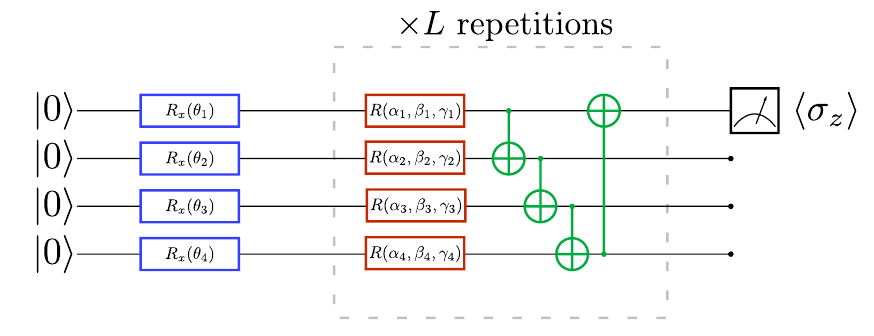
\includegraphics[width=\textwidth]{angleemb.png}
        \caption{\small Circuito cuántico con Angle Embedding}
      \end{figure}
    \end{column}
  \end{columns}
\end{frame}

% ===================================================================
% SECCIÓN 3: ARQUITECTURA DEL CIRCUITO
% ===================================================================
\section{Arquitectura del Circuito}

% ----- Diapositiva: Diseño del Circuito QML -----
\begin{frame}{Diseño del circuito}
  \begin{columns}
    \begin{column}{0.55\textwidth}
      \begin{block}{Componentes principales}
        \begin{itemize}
          \item \texttt{device}: \alert{lightning.gpu} (simulador)
          \item 16 qubits para características del jet
          \item 4 capas de entrelazamiento
          \item Medición del observable $\langle Z_0\rangle$
        \end{itemize}
      \end{block}
      \begin{alertblock}{Implementación}
        \begin{itemize}
          \item Framework: PennyLane + PyTorch
          \item Optimizador: Adam ($lr=0.02$)
        \end{itemize}
      \end{alertblock}
    \end{column}
    \begin{column}{0.45\textwidth}
      \begin{figure}
        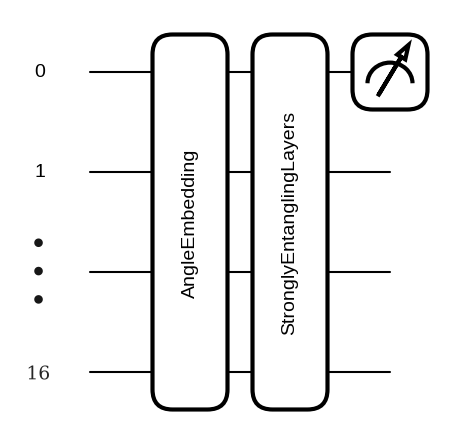
\includegraphics[width=\textwidth]{circuito.png}
        \caption{Estructura del circuito}
      \end{figure}
    \end{column}
  \end{columns}
\end{frame}

% ----- Diapositiva: Capas de Entrelazamiento Fuerte -----
\begin{frame}{Capas de entrelazamiento fuerte}
  \begin{columns}
    \begin{column}{0.6\textwidth}
      \begin{block}{Estructura por capa}
        \begin{enumerate}
          \item \textbf{Rotaciones locales}
            \begin{itemize}
              \item $RX(\theta)$, $RY(\phi)$, $RZ(\lambda)$
              \item Parámetros entrenables
            \end{itemize}
          \item \textbf{Entrelazamiento}
            \begin{itemize}
              \item Puertas CNOT y CZ
            \end{itemize}
        \end{enumerate}
      \end{block}
    \end{column}
    \begin{column}{0.4\textwidth}
      \begin{figure}
        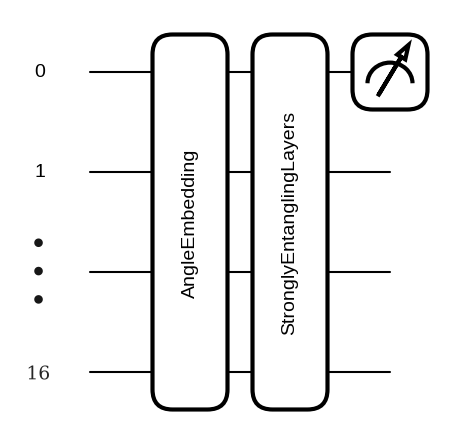
\includegraphics[width=\textwidth]{circuito.png}
        \caption{Estructura del circuito}
      \end{figure}
    \end{column}
  \end{columns}
\end{frame}

% ----- Diapositiva: ¿Dónde está el Aprendizaje? -----
\begin{frame}{¿Dónde está el Aprendizaje?}
  \begin{columns}
    \begin{column}{0.49\textwidth}
      \begin{block}{Angle Embedding (Fijo )}
        \begin{itemize}
          \item Codifica las 16 features del jet
          \item Solo depende de los datos de entrada
        \end{itemize}
        $$|\psi\rangle = \bigotimes_i R_Y(\theta_i^{\text{jet}})|0\rangle$$
      \end{block}
    \end{column}
    
    \begin{column}{0.49\textwidth}
      \begin{alertblock}{Capas (Entrenable )}

        \begin{itemize}
          \item 4 capas de rotaciones $R(\alpha, \beta, \gamma)$
          \item 16 qubits $\times$ 3 ángulos = 48 parámetros/capa
        \end{itemize}
        $$U(\vec{w}) = \prod_{l=1}^{4} \left[\prod_i R_i^l(\vec{w}_i^l) \cdot \text{CNOT}\right]$$
      \end{alertblock}
    \end{column}
  \end{columns}
  
  \vspace{1em}
  \begin{center}
    \Large
    $\hat{y} = \langle 0 | U^\dagger(\vec{w}) \cdot \sigma_z \cdot U(\vec{w}) | \psi_{\text{data}} \rangle$
    
    \textcolor{red}{$\uparrow$ Aquí se optimiza $\vec{w}$ para minimizar el error}
  \end{center}
\end{frame}

% ----- Diapositiva: Correlaciones Cuánticas -----
\begin{frame}{Correlaciones cuánticas en el circuito}
  \begin{columns}
    \begin{column}{0.6\textwidth}
      \vspace{-0.2em}
      \begin{alertblock}{Observables de medición}
        \[ \langle Z_0 \rangle = \bra{\psi} Z_0 \ket{\psi} \in [-1,1] \]
        \begin{itemize}
          \item $+1$: b-jet
          \item $-1$: anti-b-jet
        \end{itemize}
      \end{alertblock}
    \end{column}
    \begin{column}{0.38\textwidth}
      \begin{figure}
        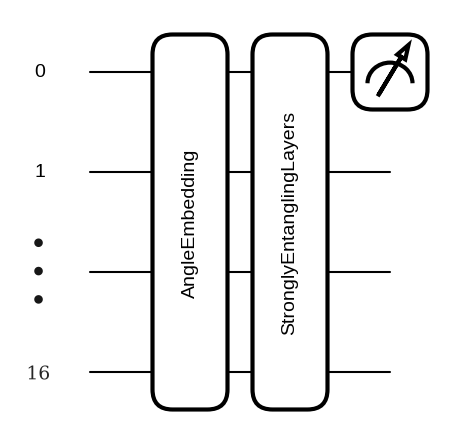
\includegraphics[width=\textwidth]{circuito.png}
        \caption{Estructura del circuito}
      \end{figure}
    \end{column}
  \end{columns}
\end{frame}

% ===================================================================
% SECCIÓN 4: METODOLOGÍA
% ===================================================================
\section{Metodología}

% ----- Diapositiva: Flujo de Trabajo -----
\begin{frame}{Flujo de trabajo}
  \begin{columns}
    \begin{column}{0.48\textwidth}
      \begin{block}{Preprocesamiento}
        \begin{enumerate}
          \item Carga de histogramas ROOT
          \item Normalización con arctan
          \item Selección de 16 características
        \end{enumerate}
      \end{block}
      \vspace{-0.2em}
      \begin{block}{Modelos}
        \begin{itemize}
          \item \textbf{QML}: 16 qubits, 4 capas SEL
          \item \textbf{DNN}: 16-64-32-1, ReLU/tanh
        \end{itemize}
      \end{block}
    \end{column}
    \begin{column}{0.48\textwidth}
      \begin{alertblock}{Entrenamiento}
        \begin{itemize}
          \item Optimizador: Adam
          \item Learning rate: 0.02
          \item Épocas: 10
        \end{itemize}
      \end{alertblock}
      \vspace{-0.2em}
      \begin{block}{Evaluación}
        \begin{itemize}
          \item AUC-ROC
          \item Tagging Power
          \item Análisis por \texorpdfstring{$p_T$}{pT}
        \end{itemize}
      \end{block}
    \end{column}
  \end{columns}
\end{frame}

% ===================================================================
% SECCIÓN 5: RESULTADOS
% ===================================================================
\section{Resultados}

% ----- Diapositiva: Comparación de Rendimiento -----
\begin{frame}{Comparación de rendimiento}
  \begin{columns}
    \begin{column}{0.44\textwidth}
      \begin{block}{Datasets analizados}
        \begin{itemize}
          \item Zbb\_LowPT (\texorpdfstring{$p_T < 20$}{pT < 20} GeV)
          \item Zbb\_HighPT (\texorpdfstring{$p_T \geq 20$}{pT >= 20} GeV)
          \item Zp\_M30\_LowPT
          \item Zp\_M100\_LowPT
        \end{itemize}
      \end{block}
      \vspace{-0.2em}
      \begin{alertblock}{Métricas clave}
        \begin{itemize}
          \item AUC: QML vs DNN
          \item Tagging Power (\texorpdfstring{$\epsilon_{\text{tag}}$}{epsilon})
        \end{itemize}
      \end{alertblock}
    \end{column}
    \begin{column}{0.54\textwidth}
      \begin{figure}
        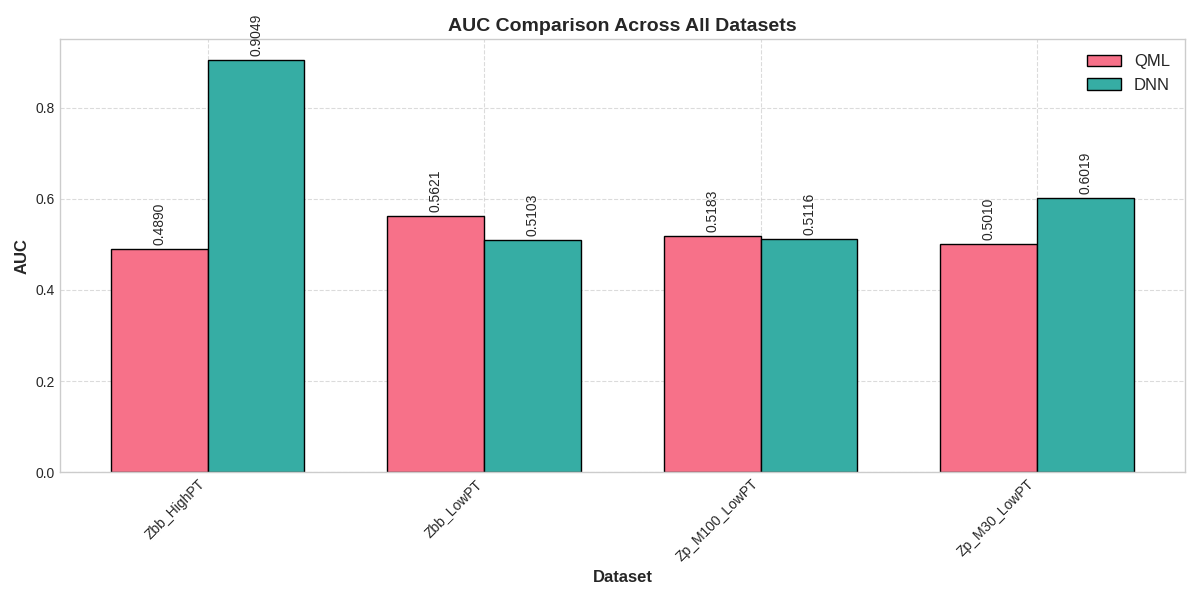
\includegraphics[width=\textwidth]{resumen_hmmm/auc_all_datasets.png}
        \caption{\small Comparativa AUC}
      \end{figure}
    \end{column}
  \end{columns}
\end{frame}

% ----- Diapositiva: Análisis por Régimen -----
\begin{frame}{Análisis por régimen de \texorpdfstring{$p_T$}{pT}}
  \begin{columns}
    \begin{column}{0.45\textwidth}
      \begin{alertblock}{Observaciones}
        \begin{itemize}
          \item DNN superior en alto \texorpdfstring{$p_T$}{pT}
          \item Brecha menor en bajo \texorpdfstring{$p_T$}{pT}
          \item Potencial para mejora en QML
          \item Consideracion del tamaño muestral
        \end{itemize}
      \end{alertblock}
    \end{column}
    \begin{column}{0.53\textwidth}
      \begin{figure}
        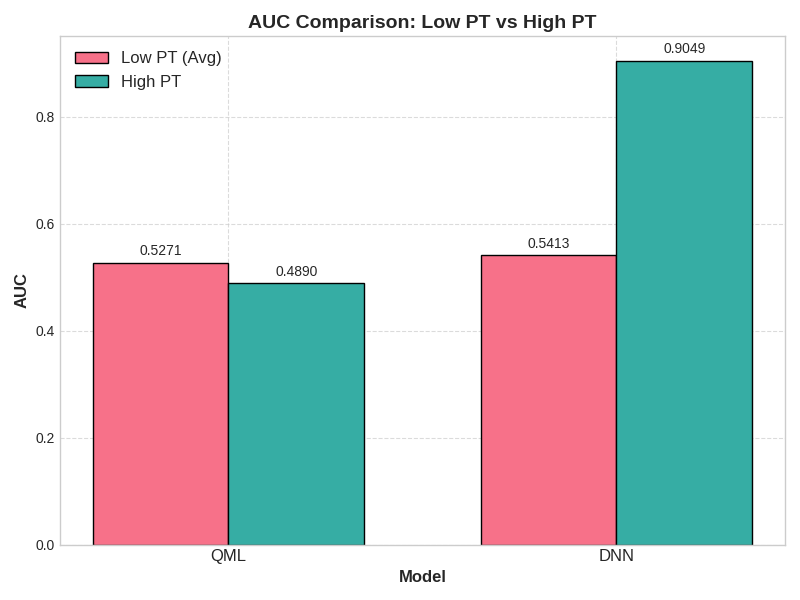
\includegraphics[width=\textwidth]{resumen_hmmm/auc_low_vs_high_pt.png}
        \caption{\footnotesize Rendimiento en función del \texorpdfstring{$p_T$}{pT}}
      \end{figure}
    \end{column}
  \end{columns}
\end{frame}

% ----- Diapositiva: Tagging Power -----
\begin{frame}{Tagging power}
  \begin{columns}
    \begin{column}{0.48\textwidth}
      \begin{block}{\texorpdfstring{$\epsilon_{\text{tag}} = \epsilon_{\text{eff}}(2a-1)^2$}{Tagging power Formula}}
        \begin{itemize}
          \item \texorpdfstring{$\epsilon_{\text{eff}}$}{epsilon\_eff}: eficiencia de tagging
        \end{itemize}
      \end{block}
      \vspace{-0.2em}
      \begin{alertblock}{Resultados}
        \begin{itemize}
          \item Z': desafío para ambos
        \end{itemize}
      \end{alertblock}
    \end{column}
    \begin{column}{0.5\textwidth}
      \begin{figure}
        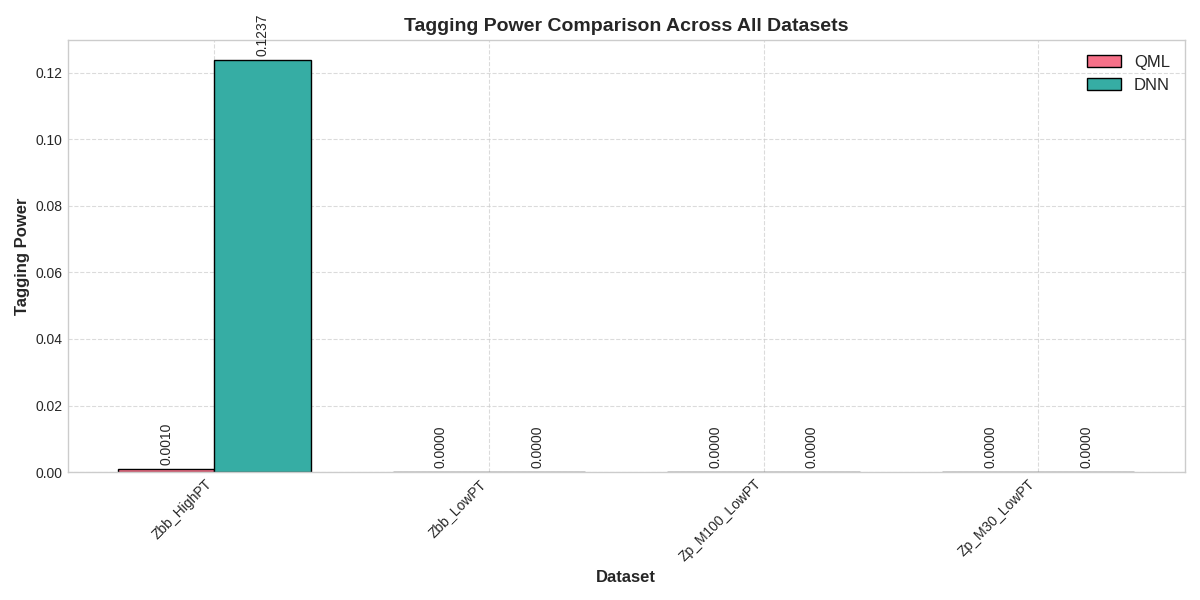
\includegraphics[width=\textwidth]{resumen_hmmm/tagging_power_all_datasets.png}
        \caption{\small Tagging Power por dataset}
      \end{figure}
    \end{column}
  \end{columns}
\end{frame}

% ===================================================================
% SECCIÓN 6: CONCLUSIONES
% ===================================================================
\section{Conclusiones}

% ----- Diapositiva: Hallazgos Principales -----
\begin{frame}{Hallazgos principales}
  \begin{columns}
    \begin{column}{0.43\textwidth}
      \begin{block}{Observaciones}
        \begin{itemize}
          \item Mayor variabilidad en bajo \texorpdfstring{$p_T$}{pT}
          \item Potencial para mejora
        \end{itemize}
      \end{block}
      \vspace{-0.3em}
      \begin{alertblock}{Desafíos}
        \begin{itemize}
          \item Muestra limitada (1000 eventos)
          \item El regimen de baja energia del Z'
        \end{itemize}
      \end{alertblock}
    \end{column}
    \begin{column}{0.55\textwidth}
      \vspace{-0.3em}
      \begin{figure}
        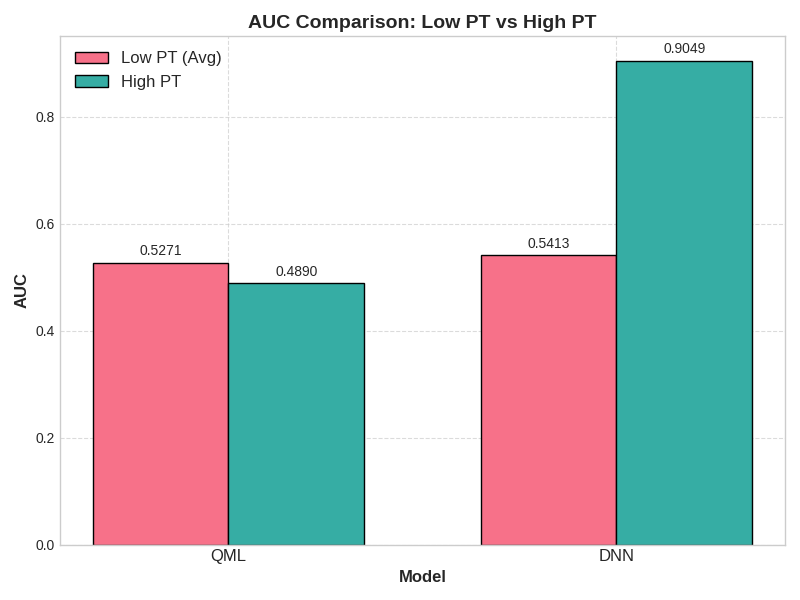
\includegraphics[width=0.85\textwidth]{resumen_hmmm/auc_low_vs_high_pt.png}
        \caption{\footnotesize Resumen de rendimiento}
      \end{figure}
    \end{column}
  \end{columns}
\end{frame}

% ----- Diapositiva: Perspectivas Futuras -----
\begin{frame}{Perspectivas futuras}
  \begin{columns}
    \begin{column}{0.48\textwidth}
      \begin{block}{Mejoras técnicas}
        \begin{itemize}
          \item Arquitecturas más profundas
          \item Embeddings alternativos
          \item Optimización de hiperparámetros
        \end{itemize}
      \end{block}
      \vspace{-0.2em}
      \begin{alertblock}{Nuevas direcciones}
        \begin{itemize}
          \item Variables específicas para QML
          \item Análisis de correlaciones cuánticas
          \item Hardware
        \end{itemize}
      \end{alertblock}
    \end{column}
    \begin{column}{0.48\textwidth}
      \begin{block}{Impacto potencial}
        \begin{itemize}
          \item Mejor discriminación en bajo \texorpdfstring{$p_T$}{pT}
          \item Acceso a nueva física
        \end{itemize}
      \end{block}
    \end{column}
  \end{columns}
\end{frame}

% ===================================================================
% SECCIÓN 7: REFERENCIAS
% ===================================================================
\section{Referencias}

% ----- Diapositiva: Referencias y Recursos -----
\begin{frame}{Referencias y recursos}
  \vspace{-1.3em}
  \begin{block}{Artículos principales}
    \begin{thebibliography}{3}
      \bibitem{Exposicion}
        A. Gianelle et al., "First implementation of QML for b-jet tagging at LHCb", 2021.
        \href{https://indico.cern.ch/event/1053287/contributions/4442055/attachments/2332563/3975381/qml@lhcb_zuliani.pdf}{\beamerbutton{Presentación}}
      
      \bibitem{angle_embedding}
        A. Gianelle et al., "QML for b-jet charge identification", 2022.
        \href{https://arxiv.org/pdf/2202.13943}{\beamerbutton{Artículo}}
      
      \bibitem{Representacion}
        "Quantum Neural Networks explained", 2024.
        \href{https://youtu.be/xL383DseSpE}{\beamerbutton{Video Tutorial}}
    \end{thebibliography}
  \end{block}
  
  \begin{alertblock}{Código}
    \vspace{-1em}
    \begin{columns}
      \begin{column}{0.65\textwidth}
        \begin{itemize}
          \item Repo GitHub: \href{https://github.com/JuanJ27/LowPt-Jet-Qml/tree/main}{github.com/JuanJ27/LowPt-Jet-Qml}
        \end{itemize}
      \end{column}
      \begin{column}{0.35\textwidth}
        \begin{figure}
          \centering
          \includegraphics[width=0.65\textwidth]{qrcode_github.com.png}
        \end{figure}
      \end{column}
    \end{columns}
  \end{alertblock}
\end{frame}

\end{document}
